\usepackage{etex}
\reserveinserts{28}
\usepackage{euler}
%\usepackage{picins}
\usepackage{xkeyval}[2005/11/25]
\usepackage{eso-pic}
\usepackage{graphicx}
\usepackage{fp}
\usepackage{tikz}
\usetikzlibrary{calc,positioning}
\usetikzlibrary{decorations.pathmorphing}
\usetikzlibrary{decorations.pathreplacing} 
\usetikzlibrary{decorations.shapes} 
\usetikzlibrary{shadows}
\usetikzlibrary{arrows}
\usetikzlibrary{shapes,snakes,shapes.geometric,shapes.misc}
\usepackage{multicol}
\usepackage{amsmath,amsfonts,amssymb}
\usepackage{float}
\usepackage{array,booktabs ,tabularx,multirow}
\usepackage[most]{tcolorbox}
\usepackage[top=1cm,bottom=0cm,left=1cm,right=1cm]{geometry}
%\usepackage{fancyhdr}
%\usepackage{xlop}
\usepackage{environ}
\usepackage{etoolbox}
\usepackage{fontspec}
\usepackage{arabxetex}
\newfontfamily\arabicfont[Script=Arabic , Scale=1.5]{ae_Sindibad}


%%%%%%%%%%%%%%%%%%%%%%%%%%%%%%%%%%%%%%%%%%%%%%%%%%%%%%%%%%%
\begingroup\lccode`~=`_ \lowercase{\endgroup\let~\sb}
\AtBeginDocument{\mathcode`\_=\string"8000 \catcode`\_=12 }

\begingroup\lccode`~=`^ \lowercase{\endgroup\let~}\sp
\begingroup\lccode`~=`_ \lowercase{\endgroup\let~}\sb
\AtBeginDocument{\mathcode`^=\string"8000  \catcode`\^=11 \mathcode`_=\string"8000  \catcode`\_=12 }
%%%%%%%%%%%%%%%%%%%%%%%%%%%%%%%%%%%%%%%%%%%%%%%%%%%%%%%%%%%%%%%
\tikzset{
    mybox/.style={
        draw=red, fill=blue!20, very thick,
        rectangle, rounded corners, inner sep=10pt, inner ysep=20pt
    },
    fancytitle/.style={
            draw=red, fill=blue!20, text=black, rectangle, rounded corners
    }
}
%%%%%%%%%%%%%%%%%%%%%%%%%%%%%%%%%%%%%%%%%%%%%%%%%%%%%%%%%%%
\NewEnviron{exercice}{%
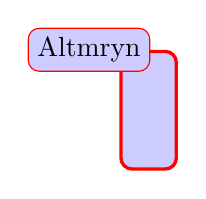
\begin{tikzpicture}
\node [mybox] (box){%
\begin{minipage}{0.9\textwidth}
\BODY
\end{minipage}
};
\node[fancytitle, left=10pt] at (box.north east) {\textarab{Altmryn}};
\end{tikzpicture}%
}
%----------------------------------------...les compteurs..... ----------------------------------------------------------------------%
\newcounter{i}
\setcounter{i}{1}
\newcounter{k}
\setcounter{k}{1}
%----------------------------------------------------------\cadre[x=... ,y=.....,  ]------------------------------------------------------%

% \cadre[			shadow (bool�en),
%					lw = , (�paisseur du trait, en pt)
%					style = , (dashed ou dotted)
%					x = abscisse du sommet en bas � gauche,
%					y = ordonn�e du sommet en bas � gauche,
%					xshadow = d�calage selon x de l'ombre,
%					yshadow = d�calage selon y de l'ombre,
%					color = couleur du cadre,
%					colorshadow = couleur de l'ombre,
%					decoration = nom de la d�coration,
%					doubleline (bool�en) pour pstricks
%				  ]
\makeatletter
\define@cmdkey [PAS] {cadre} {x}{}
\define@cmdkey [PAS] {cadre} {y}{}
\define@cmdkey [PAS] {cadre} {decoration}{}
\define@cmdkey [PAS] {cadre} {shape}{}
\define@cmdkey [PAS] {cadre} {lw}{}
\define@cmdkey [PAS] {cadre} {xshadow}{}
\define@cmdkey [PAS] {cadre} {yshadow}{}
\define@cmdkey [PAS] {cadre} {bordercolor}{}
\define@cmdkey [PAS] {cadre} {incolor}{}
\define@cmdkey [PAS] {cadre} {shadowcolor}{}
\define@cmdkey [PAS] {cadre} {style}{}
\define@boolkey[PAS] {cadre} {shadow}[true]{}
\define@boolkey[PAS] {cadre} {doubleline}[true]{}

\presetkeys    [PAS] {cadre} {	shadow = false,
								lw = 2,
								x = 0.2,
								y = 0.2,
								xshadow =- 0.35,
								yshadow =0.2,
								bordercolor = black,
								incolor = white,
								shadowcolor = gray,
								style = ,
								doubleline = false,
								decoration = , 
								shape = }{}

\newcommand*{\cadre}[1][]{\pasCadre[#1]}

\def\pasCadre[#1]{
	\setkeys[PAS]{cadre}{#1}
	
	\AddToShipoutPicture
	{
		\put(\LenToUnit{\cmdPAS@cadre@x cm},\LenToUnit{\cmdPAS@cadre@y cm})
		{
				\ifPAS@cadre@doubleline
					\edef\dl{double}
				\else
					\edef\dl{}
				\fi
				\begin{tikzpicture}[decoration={\cmdPAS@cadre@decoration,shape=\cmdPAS@cadre@shape}]
					\pgfsetlinewidth{\cmdPAS@cadre@lw pt}
					\ifPAS@cadre@shadow
						\filldraw[
						decorate,
						fill=\cmdPAS@cadre@incolor,
						draw=\cmdPAS@cadre@bordercolor,
						style=\cmdPAS@cadre@style,
						drop shadow={fill=\cmdPAS@cadre@shadowcolor,shadow xshift=\cmdPAS@cadre@xshadow cm,shadow yshift=-\cmdPAS@cadre@yshadow cm},
						\dl] (0,0) -- (0,\paperheight-2*\cmdPAS@cadre@y cm) -- (\paperwidth-2*\cmdPAS@cadre@x cm,\paperheight-2*\cmdPAS@cadre@y cm) -- (\paperwidth-2*\cmdPAS@cadre@x cm,0) -- cycle;
					\else
						\filldraw[
						decorate,
						fill=\cmdPAS@cadre@incolor,
						draw=\cmdPAS@cadre@bordercolor,
						style=\cmdPAS@cadre@style,
						\dl] (0,0) -- (0,\paperheight-2*\cmdPAS@cadre@y cm) -- (\paperwidth-2*\cmdPAS@cadre@x cm,\paperheight-2*\cmdPAS@cadre@y cm) -- (\paperwidth-2*\cmdPAS@cadre@x cm,0) -- cycle;
					\fi
				\end{tikzpicture}
		}
	}
}

\def\nocadre{\ClearShipoutPicture}
%------------------\entete---------------------------------%
 \catcode`\_=11 
\newcommand{\entete}{%
\noindent
\begin{tabularx}{\textwidth}{r X r}
\toprule
\textarab{AlmdT AlzmnyT :  sA`tAn} &
  \LARGE\centering \textarab{Al-'imt.hAn Al|m|.hly Al|m|w.hd} &
  \textarab{'i`dAdyT `bd Alkrym Alx.tAby } \\
\textarab{AldwrT : $II$}&
  \Large\centering \textarab{fy m|AdT AlryA.dyAt} &
  \textarab{nyAbT tAwryrt} \\
\textarab{Alm`Aml : $3$} &
  \centering \textarab{AlsnT Al_tAl_tT 'i`dAdy} &
  \textarab{dabdw} \\
\bottomrule
\end{tabularx}
} \catcode`\_=8
%--\exo[bareme,bar=...]{........}------------------------------%

\define@cmdkey[EX]{exo}{bar}{}
\define@boolkey[EX]{exo}{bareme}[true]{}
\presetkeys[EX]{exo}{bar= ,bareme=false}{}
\newcommand{\exo}[2][]{
\setkeys[EX]{exo}{#1}
\setcounter{k}{1}
\tikzstyle{mybox} = [ draw, very thick,rounded corners=3mm, inner sep=10pt, inner ysep=10pt]
\tikzstyle{fancytitle} =[fill=white, text=black,inner ysep=0pt,inner xsep=2pt]
\noindent
\begin{tikzpicture}
\node [mybox] (box){%
    \begin{minipage}{0.88\linewidth}
        #2 
    \end{minipage}
};
\node[fancytitle, left=10pt] at (box.north east) {{\large \arabic{i}\textarab{Altmryn}}};
\ifEX@exo@bareme
\node[fancytitle] at (box.north){\textarab{nq.t} \cmdEX@exo@bar };
\fi
\end{tikzpicture}%
\stepcounter{i}
}

%----------\devoir[niv=... , num=..., date=..., ds=...]----------%

\define@cmdkey[EX]{devoir}{niv}{}
\define@cmdkey[EX]{devoir}{num}{}
\define@cmdkey[EX]{devoir}{date}{}
\presetkeys[EX]{devoir}{niv=$3$,num=$1$,date=??/??/????}{}
\newcommand{\devoir}[1][]{
\setkeys[EX]{devoir}{#1}
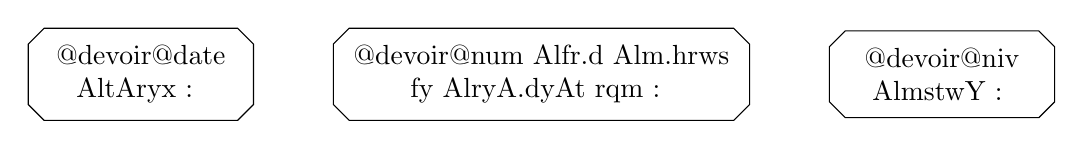
\begin{tikzpicture}
\node [draw,shape=chamfered rectangle] (box1){%
    \begin{minipage}{0.2\textwidth}
      \center \cmdEX@devoir@date \textarab{AltAryx :{} }
    \end{minipage}
};
\node [draw,shape=chamfered rectangle] (box2)[right=of box1]{%
    \begin{minipage}{0.4\textwidth}
       \center\cmdEX@devoir@num \textarab{Alfr.d Alm.hrws fy AlryA.dyAt rqm :{} }
    \end{minipage}
};
\node [draw,shape=chamfered rectangle] (box3)[right=of box2]{%
    \begin{minipage}{0.2\textwidth}
 \center\cmdEX@devoir@niv \textarab{AlmstwY :{} }     
    \end{minipage}
};
\end{tikzpicture}%
}
%------------------------------------------------\serie[titre=..]-----------------------------------------------------------------------------%

\define@cmdkey[EX]{serie}{titre}{}
\presetkeys[EX]{serie}{titre=\textarab{`nwAn Aldrs}}{}
\newcommand{\serie}[1][]{
\setkeys[EX]{serie}{#1}
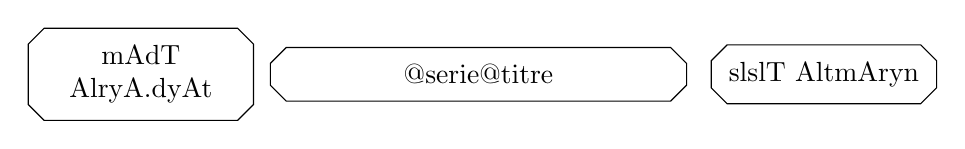
\begin{tikzpicture}
\node [draw,shape=chamfered rectangle] (box1){%
    \begin{minipage}{0.20\textwidth}
       \center\textarab{mAdT AlryA.dyAt}
    \end{minipage}
};
\node [draw,shape=chamfered rectangle] (box2)[right=0.2cm of box1]{%
    \begin{minipage}{0.40\textwidth}
      \center\cmdEX@serie@titre
    \end{minipage}
};
\node [draw,shape=chamfered rectangle] (box3)[right=0.3cm of box2]{%
    \begin{minipage}{0.20\textwidth}
   \center\textarab{slslT AltmAryn}
    \end{minipage}
};
\end{tikzpicture}%
}
\makeatother